\chapter{What is a Proof?}
\begin{pr}\leavevmode
    \begin{enumerate}[label=\textbf{(\alph*)}]
        \item \label{1.a.sec1} Colors of the triangles are arbitrary since I
        do not remember the exact ones in the text.
        \vspace{1cm}

        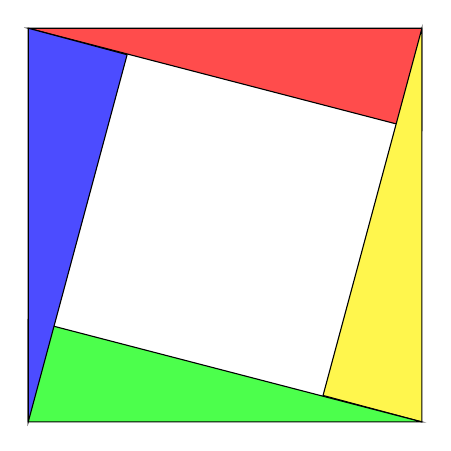
\begin{tikzpicture}
            \draw[fill=red!70] (0,0) -- (5,0) -- ++(-90:1.3) -- cycle;
            \draw[fill=yellow!70] (5,0) -- (5,-5) -- ++(165: 1.3) -- cycle;
            \draw[fill=green!70] (5,-5) -- (0,-5) -- ++(90:1.3) -- cycle;
            \draw[fill=blue!70] (0,-5) -- (0,0) -- ++(-15:1.3) -- cycle;
        \end{tikzpicture}

        \vspace{1.5\baselineskip}
        The middle square is a square of $(b-a) \times (b-a)$

        \item \label{1.b.sec1} $[$\note{Possible Errata:} Arrange the same shapes so they form
        two rectangles, both $a \times b$.$]$

        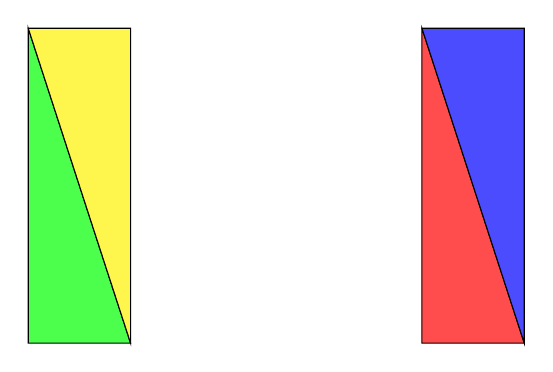
\begin{tikzpicture}
            \begin{scope}
                \draw[fill=green!70] (0,0) -- ++(0,-4) -- ++(1.3,0) -- cycle;
                \draw[fill=yellow!70] (0,0) -- ++(1.3,0) -- ++(0,-4) -- cycle;
            \end{scope}
            \begin{scope}[xshift=5cm]
                \draw[fill=red!70] (0,0) -- ++(0,-4) -- ++(1.3,0) -- cycle;
                \draw[fill=blue!70] (0,0) -- ++(1.3,0) -- ++(0,-4) -- cycle;
            \end{scope}
        \end{tikzpicture}

        We prove by construct a chain of iffs.
        \begin{IEEEeqnarray*}{C'rCl}
            & (b - a)^2 & = & c^2 - 2ab \\
            \Leftrightarrow & a^2 + b^2 - 2ab & = & c^2 - 2ab \\
            \Leftrightarrow & a^2 + b^2 & = & c^2 \\
        \end{IEEEeqnarray*}

        \item The equation would still hold true since $a = b$ is not
        a requirement for the proof. In fact, note that if $a = b$,
        the area of the bigger square in \ref{1.a.sec1} will now be
        exactly equal to the sum of area of all triangles inside it,
        which is equal to the sum of area of two smaller squares in \ref{1.b.sec1}.
        That is, $c^2 = a^2 + b^2$.

        \item Some assumptions about right triangles, squares and lines are,
        \begin{itemize}
            \item 4 identical right triangles.
            \item For every 2 points, there is a line.
        \end{itemize}
    \end{enumerate}
\end{pr}

\begin{pr}\leavevmode
    \begin{enumerate}[label=\textbf{(\alph*)}]
        \item Mistake:
        \begin{equation*}
            \sqrt{(-1)(-1)} = \sqrt{-1}\sqrt{-1}
        \end{equation*}
        The right-hand side of this equation is undefined while the left-hand side
        is defined.
        \item Suppose $1 = -1$, then
        \begin{IEEEeqnarray*}{C'rCl}
                        & 0     & = & 0 \\
            \Rightarrow & 1^2 - 1^2 & = & 1 + 1 \\
            \Rightarrow & (1 - 1)(1 + 1) & = & 1 + 1
        \end{IEEEeqnarray*}
        At this stage, we cancel off $1 + 1$ on each side since they are non-zero, the equation
        then becomes,
        \begin{IEEEeqnarray*}{C'rCl}
            \Rightarrow & 1 - 1 & = & 1 \\
            \Rightarrow & 1 + 1 & = & 1 \\
            \Rightarrow & 2 & = & 1
        \end{IEEEeqnarray*}
        where the second equation is by the antecedent $1 = -1$. Hence, we have
        proved $2 = 1$.
        \item We shall prove the following lemma,
        \begin{lemPr}
            If $r,s > 0$, then $\sqrt{rs} = \sqrt{r}\sqrt{s}$
        \end{lemPr}
        \begin{proof}
            Assume $r,s > 0$. For every positive integer $x$, there is one $\sqrt{x} > 0$
            such that $x = (\sqrt{x})^2$; therefore,
            \begin{equation}
                (\sqrt{r})^2(\sqrt{s})^2 = rs
            \end{equation}
            By commutative and associative property of multiplication, 
            \begin{equation}
                (\sqrt{r})^2(\sqrt{s})^2 = (\sqrt{r}\sqrt{s})^2
            \end{equation}
            which leads to
            \begin{equation}
                (\sqrt{r}\sqrt{s})^2 = rs
            \end{equation}
            Since $rs > 0$, there is also one $\sqrt{rs} > 0$ such that
            $(\sqrt{rs})^2 = rs$. Therefore,
            \begin{equation}
                (\sqrt{r}\sqrt{s})^2 = (\sqrt{rs})^2
            \end{equation}
            Since $\sqrt{r}\sqrt{s} > 0$ and $\sqrt{rs} > 0$,
            we conclude
            \begin{equation}
                \sqrt{r}\sqrt{s} = \sqrt{rs}
            \end{equation}
        \end{proof}
    \end{enumerate}
\end{pr}

\begin{pr}\leavevmode
    \begin{enumerate}[label=\textbf{(\alph*)}]
        \item Mistake,
        \begin{IEEEeqnarray*}{rCl}
            3                & > & 2 \\
            3\log_{10} (1/2) & > & 2\log_{10} (1/2)
        \end{IEEEeqnarray*}
        since $\log_{10} n \;\forall  0 < n < 1$ is always negative.
        \item Wrong because all arithmetic operations must be done
        on numbers with the same currency, so that they will be in the
        same field.
        \item Since $a = b$, $a - b = 0$, and therefore we cannot
        cancel $a - b$ on both sides since we cannot divide each side by $0$.
    \end{enumerate}
\end{pr}

\begin{pr}
    The questionable step is from step 2 to step 3, namely,
    \begin{IEEEeqnarray*}{rCl}
        a + b & \overset{?}{\geq} & 2\sqrt{ab} \\
        a^2 + 2ab + b^2 & \overset{?}{\geq} & 4ab
    \end{IEEEeqnarray*}

    Assume that $a, b < 0$. Then even though the first inequality
    is false, the second inequality is true, which will lead to all
    subsequent inequalities to be true. Therefore, we have just ``proved''
    that arithmetic mean is at least as large as geometric mean for
    all negative numbers $a, b$!

    To fix this,
    \begin{IEEEeqnarray*}{rCl}
        \dfrac{a + b}{2} & \geq & \sqrt{ab} \\
        a + b - 2\sqrt{ab} & \geq & 0 \\
        (\sqrt{a} - \sqrt{b})^2 & \geq & 0 \\
    \end{IEEEeqnarray*}

    This ensures that $a, b \geq 0$ for the last inequality
    to be defined.
\end{pr}